\section{Personal comments}
\label{sec:personal}

My pursue for a PhD degree is now almost one year underway, so this is a good time to reflect how I personally experienced this. When looking back, I realize that there are some areas I can improve upon. Few points for improvements are mentioned in \cref{sec:evaluation}, but first some other personal comments are listed:
\begin{itemize}
	\item I am very satisfied with my choice for Bart De Schutter as a supervisor from the DUT and I am grateful that he accepted to supervise me. I am amazed by the comprehensiveness and accurateness of his comments and his patience to explain his remarks (again and again).
	\item I am also very satisfied with my supervisors from TNO, Jan-Pieter Paardekooper and Olaf Op den Camp. The discussions I have with them are a huge inspiration for me.
	\item Most importantly, I am still enjoying my pursue for a PhD degree every day. I still feel enthusiasm when talking about my PhD and I am very eager to continue every day with my PhD and work at TNO. 
\end{itemize}

\subsection{Self-evaluation}
\label{sec:evaluation}

I am aware that there are many points for improvement. To limit the following list, I selected two points that probably deserve most attention.

\begin{itemize}
	\item \emph{Time and expectation management}: In theory, I work five days a week: two days for my PhD at the Nanyang Technological University (NTU), two days for CETRAN at the NTU, and one day for projects of TNO at the TNO office. In practice, however, my activities are a bit scattered. For example, it sometimes happends that I can only work on my PhD for one hour a day. It turned out te be hard to do proper research in one hour. Furthermore, due to internal deadlines, I sometimes have no time to work on my PhD at all for one or two weeks.
	
	I noticed that it worked best if I can focus for a longer period on my PhD, e.g., for few days or a week with no other appointments in between. This is perfectly achievable, but it needs better time and expectation management from my side. With a better planning, I think it should be possible to have more time for my PhD and to work for longer periods continuously on my PhD.
	
	Regarding expectation management, too often I say ``yes'' when asked to finish something before the end of the week, resulting in postponing my PhD work with another week. I need to be more assertive and be able to say ``no''. Furthermore, sometimes I underestimate the time I need to finish something, so I need to better estimate the time I need before saying ``yes''.
	
	\item \emph{Stakeholder management}: As with every project, several stakeholders are involved with my PhD project, see \cref{fig:stakeholders}. Regarding my work, I identified four important stakeholders, each with different demands:
	\begin{itemize}
		\item \emph{TNO Singapore}: Obtain good results with CETRAN and acquire new projects.
		\item \emph{TNO Netherlands}: Develop the methodology of generating test cases based on real-world data.
		\item \emph{CETRAN}: Develop a certification procedure for AVs.
		\item \emph{DUT}: Assuring that the work is scientifically correct and relevant.
	\end{itemize}
	The work for my PhD needs to be useful for all these stakeholders. Sometimes, the work I do is only useful for a limited number of stakeholders, which makes my work less efficient.
	
	Next to the stakeholders regarding my work, there are stakeholders that involve my personal life (see \cref{fig:stakeholders}) and that have a direct influence on my PhD project. Although I feel full support from these stakeholders regarding my PhD and my ``Singapore campaign'', it sometimes leads to conflicts.
	
	One way to improve on my stakeholder management is communicating clearly the expectations and objectives of myself and the other stakeholders among the different stakeholders. To further improve on this, I want to follow a course on stakeholder management.
\end{itemize}

\begin{figure}
	\centering
	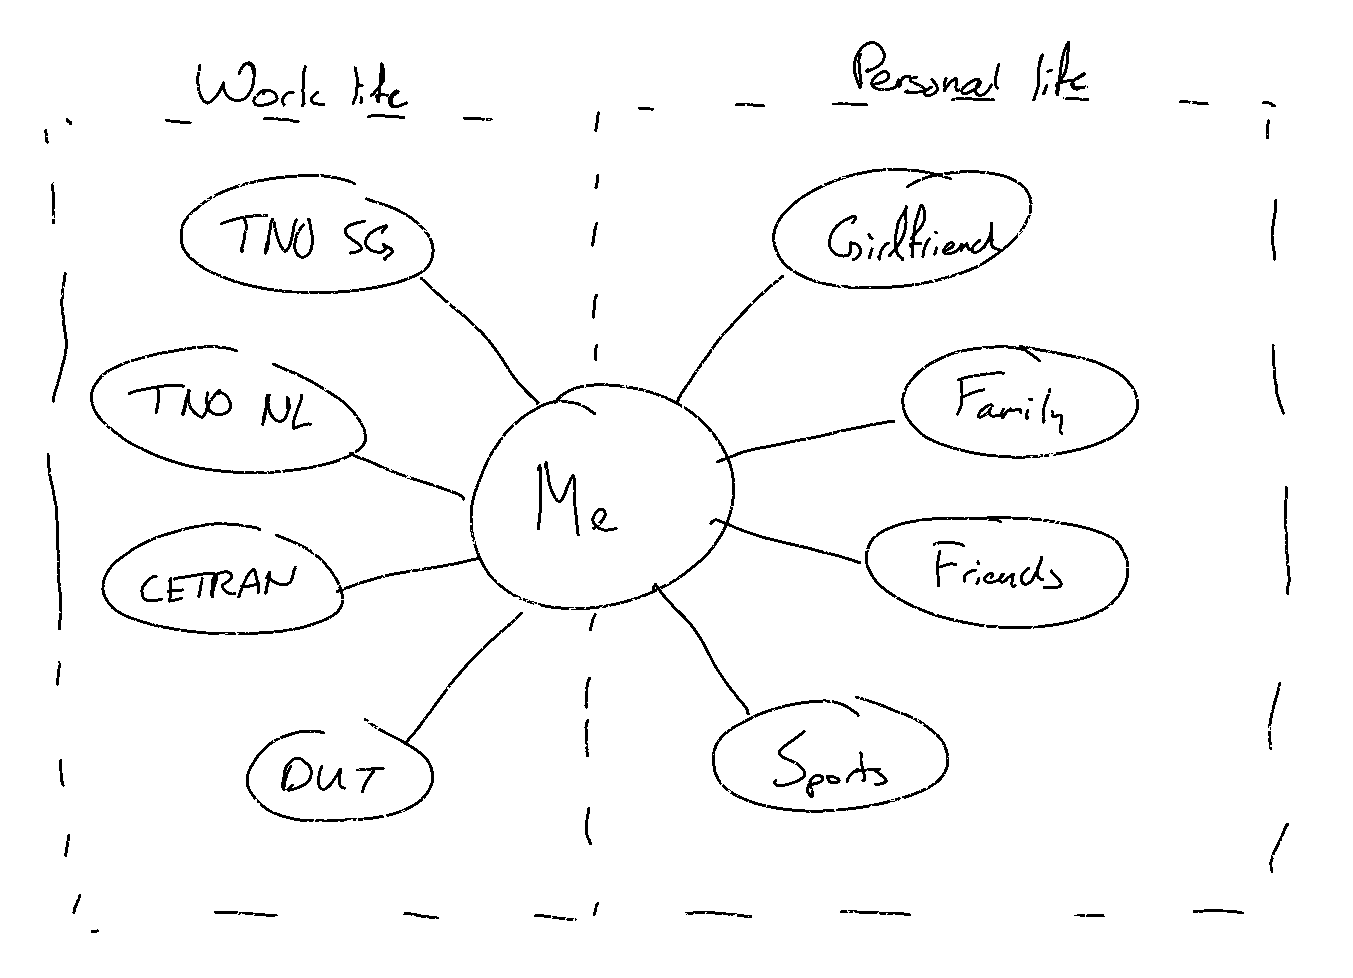
\includegraphics[width=\linewidth]{figures/stakeholders}
	\caption{Overview of the different stakeholders that are involved in my PhD project, either relating to my work or personal life.}
	\label{fig:stakeholders} 
\end{figure}

%\subsection{Graduate school}
%\label{sec:graduate school}
